%!TEX root = ../crimson_throne_book_main.tex
% 2016-06-04
\section{25 Arodus 4708}

The companions spend the night with the distraught Leroung family in the old fishery. The next morning they deliberate with the nobles on how to proceed. It is clear that the government will hunt down the Leroungs, so they'll need a place to hide. Getting them out of the city to a safe haven like Magnimar would take too much precious time, so while that option would probably be best, it is not viable at the moment. Quint suggests taking them to Glorio Arkona, but Christine Leroung does not trust the man in the least and blocks off that idea. The best alternative seems to be the rebellion. If they can locate the rebel hideout, the Leroungs could take shelter there. Christine Leroung is still fuming at the young heroes for getting her mother killed and walks out of the meeting. Only Sirtane Leroung, the late lady Eliasia's sister, retains enough clarity to talk to the party. Quint leaves the books they took from the library with her and makes for the city to try and find out where the rebels are hiding. He takes Balian with him for added security. Sjo remains in the fishery to guard the Leroung family and Puk returns to the library to see if their nightly exploits have been discovered yet. It turns out they have: numerous Gray Maidens are walking in and out of the building, obviously upset by the murder of so many of their sisters. The atmosphere crackles with nervous energy and anger.\\

Quint and Balian scout the harbor, only to come across a town crier, who announces a big parade to be held in the streets - including the palace square - around noon. He invites all citizens to attend. This parade will apparently take off in the harbor, where an enormous festive wagon is being prepared. The front of this float holds a podium and the back sports an impressive loading area with some kind of dragon-headed crane. Our friends notice the heavy-bodied new seneschal of Korvosa, the Acadamae master of Transmutation, Togomor, floating above the deck of a ship. He uses his magic to lift a humongous box out of the hold and attaches it to the dragon crane on the wagon. It is unclear what the box contains exactly, but it most certainly holds some kind of ferocious animal that growls and struggles inside the iron walls. Next a half-orc with a vicious whip leads out six large white-furred and four-armed gorillas and harnesses them up one by one to pull the vehicle. By noon a group of entertainers arrives, most of whom Quint knows as rather mediocre artists. They will form the music band that will lead the march through the city. Next several warrior-like types get off the boat: a fierce-looking ettin and ogre, a broad-shouldered human carrying two blades at his belt who moves with a grace that belies his muscular build. There are also a tall and proud Shoanti barbarian, two bugbears in armor who look like twins and an orc with a heavy halberd.\hyperref[fig:Korvosa-parade-to-reopen-the-arena-613133348]{ The two-headed giant takes up position behind the box } , the ogre follows the band and precedes the girallon train. The other humanoids climb on the podium or crane, ready to wave at the audience as they pass. \\

\begin{figure}[h]
	\centering
	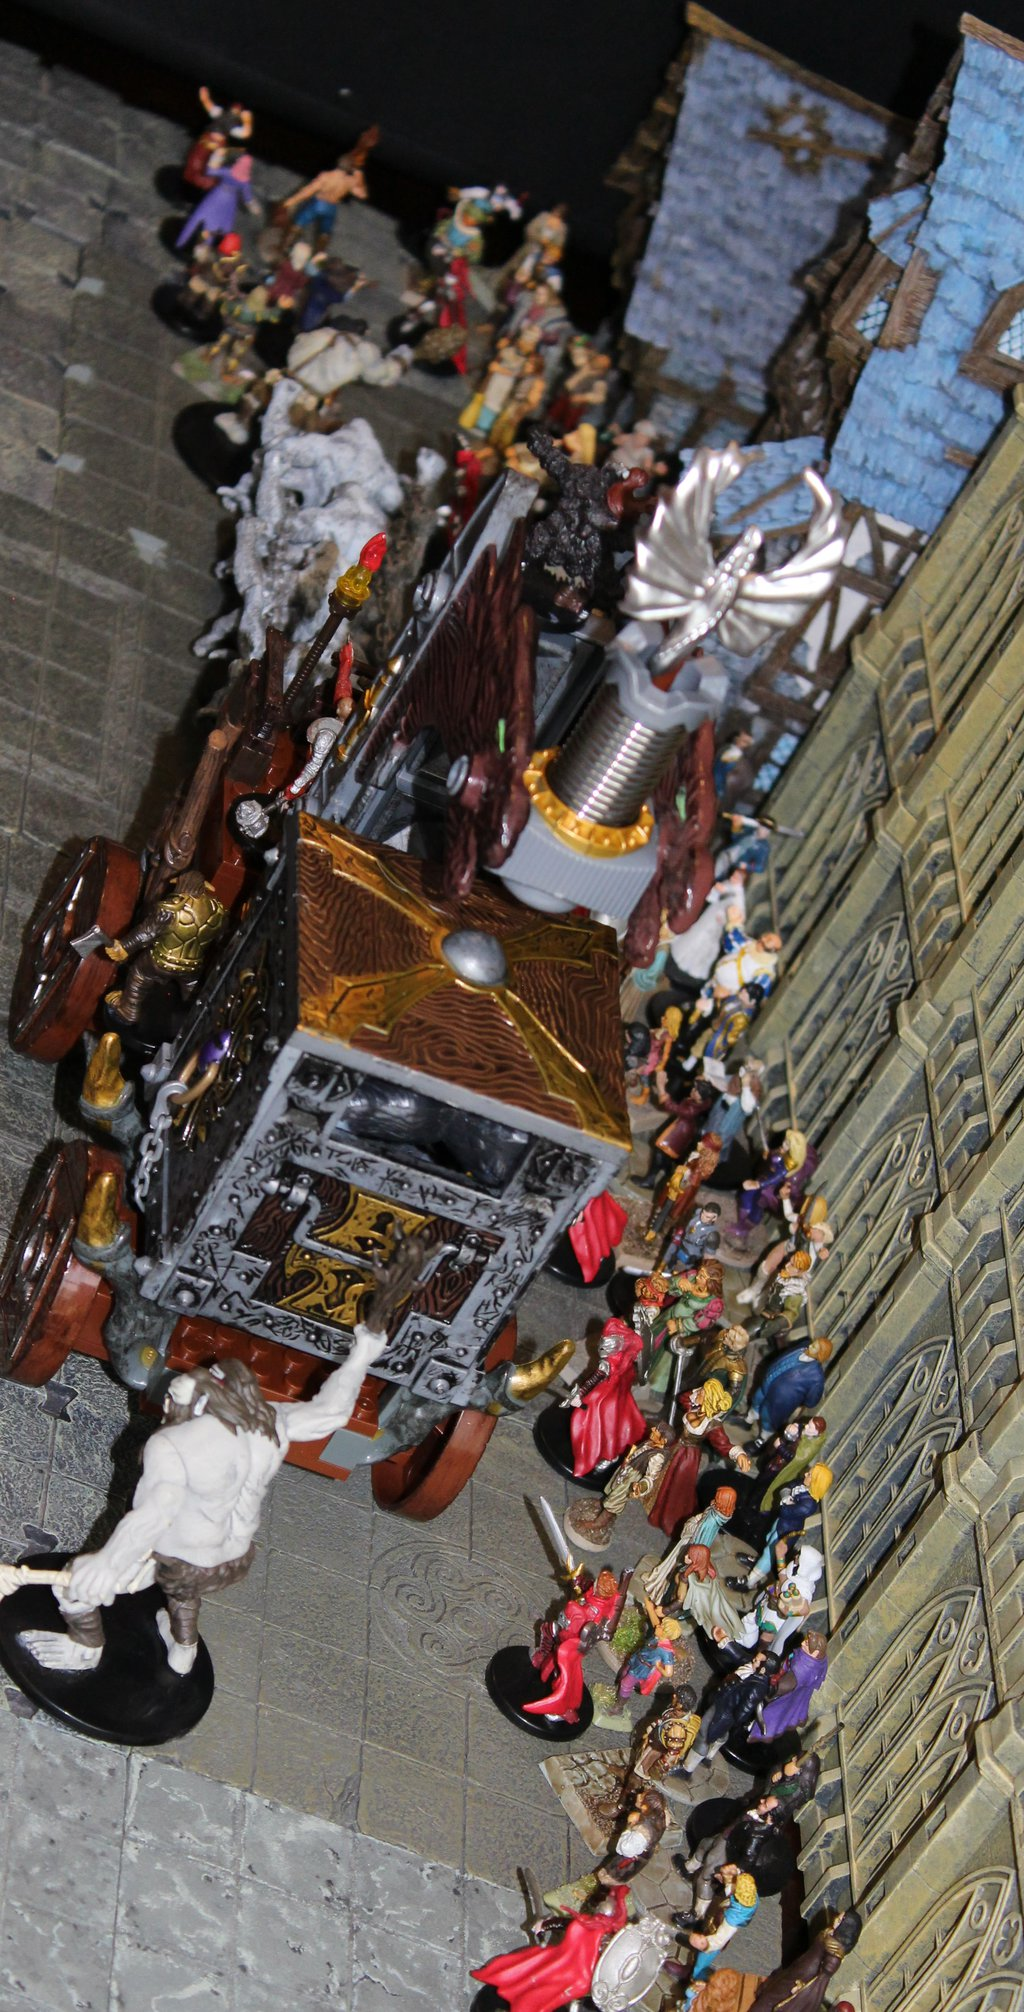
\includegraphics[width=0.39\textwidth]{images/Korvosa-parade-to-reopen-the-arena-613133348.jpg}
	\caption{Korvosa parade to reopen the arena}
	\label{fig:Korvosa-parade-to-reopen-the-arena-613133348}
\end{figure}

\hyperref[fig:Arena-parade-in-Korvosa-613132167]{ When the parade finally gets moving, a fair number of people have come out of their houses to watch. } Young boys runs about handing out flyers, announcing the reopening of the old Kendall Arena. Queen Ileosa offers her subjects the wonderful opportunity to see the greatest gladiators in Golarion fight monstrous beasts and even each other to the death. Chief among these champions of the arena is the mighty Maxor from Cheliax, the handsome human with the two blades. \\

\begin{figure}[h]
	\centering
	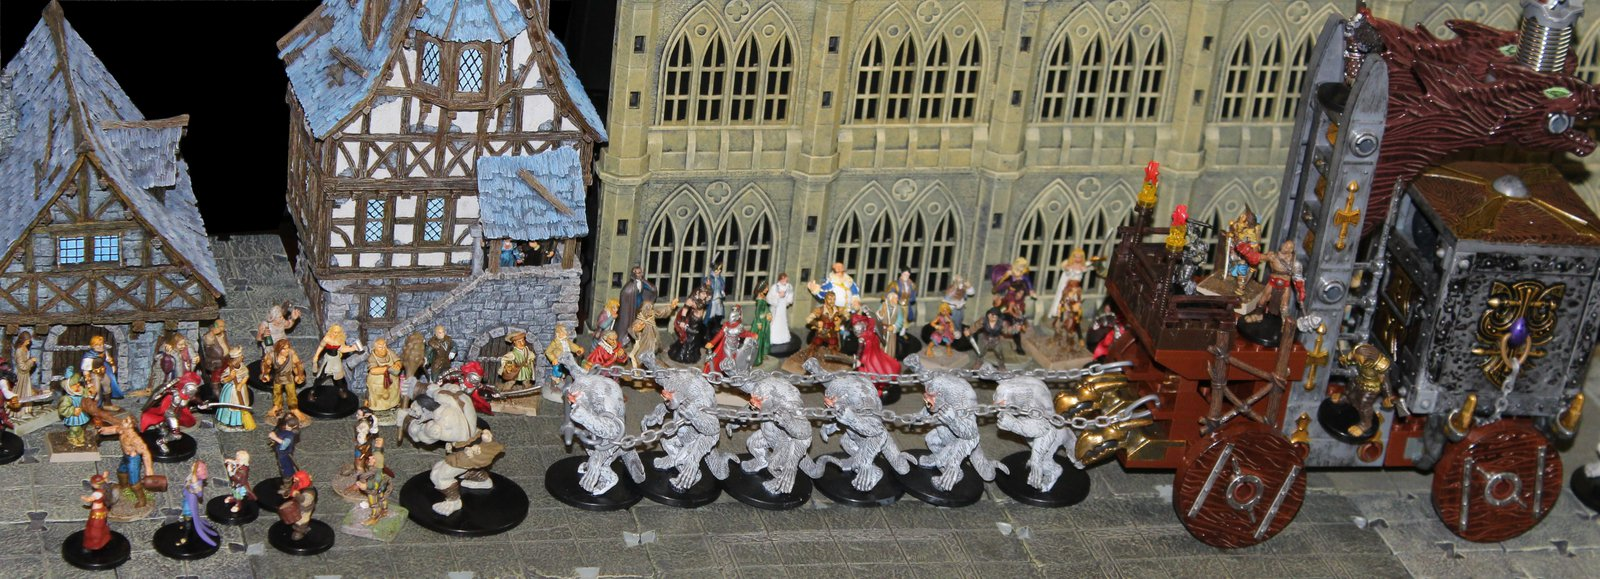
\includegraphics[width=0.39\textwidth]{images/Arena-parade-in-Korvosa-613132167.jpg}
	\caption{Arena parade in Korvosa}
	\label{fig:Arena-parade-in-Korvosa-613132167}
\end{figure}

Balian and Quint follow the parade all the way to the palace. Along the way they hook up with Puk, who has come down to see the show as well. A mild feeling of wonder and enthusiasm has taken hold of the crowd, which increases when the parade reaches the palace, where the troupe halts to greet the queen. Ileosa is standing on the palace terrace overlooking the spectacle. The band burst out in a song that turns out to be the new Korvosan hymn, honoring the city and its queen. Quint takes mental notes on the composition, so he can replay it if a future occasion calls for it. When the anthem is over, the crowd cheers wildly. Ileosa's charm offensive seems to be working, though her display of power still has to reach its climax. From behind the castle loud screeches ring out as one, then two and finally three mighty dragons rise up.\hyperref[fig:Ileosa-mother-of-dragons-613162775]{ The crowd falls silent when it sees the awe-inspiring red, blue and black winged serpents land next to the queen. } Then the buzz takes up again, leading to an overwhelming applause and cries of 'the mother of dragons'. \\

\begin{figure}[h]
	\centering
	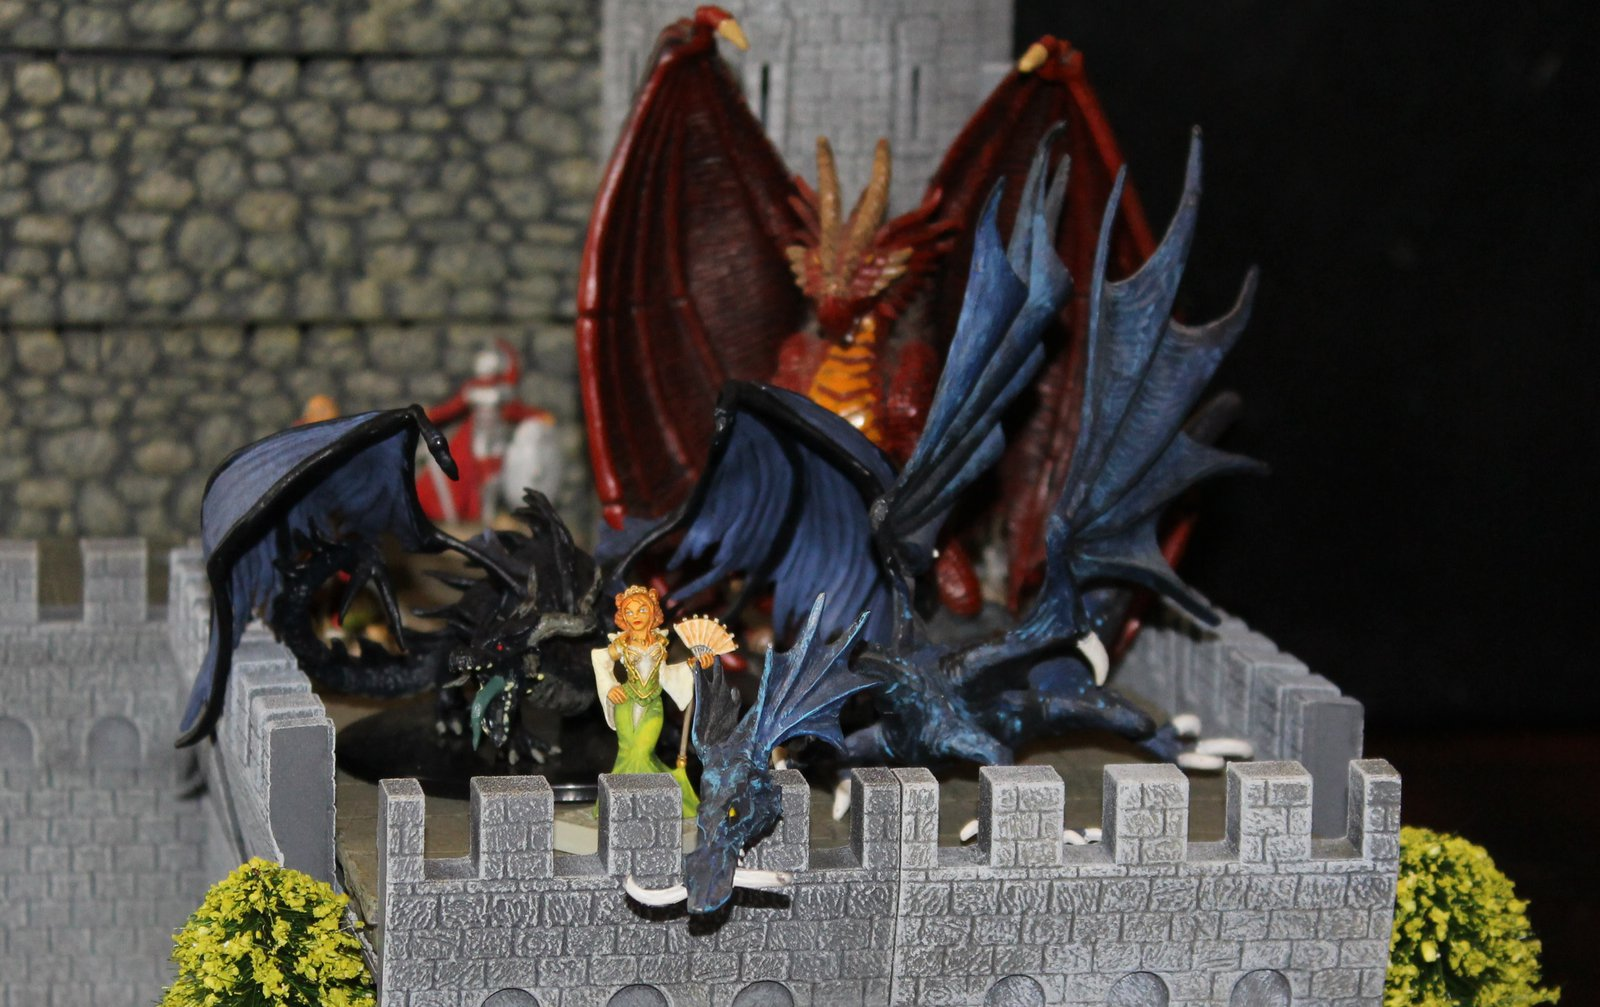
\includegraphics[width=0.39\textwidth]{images/Ileosa-mother-of-dragons-613162775.jpg}
	\caption{Ileosa, mother of dragons}
	\label{fig:Ileosa-mother-of-dragons-613162775}
\end{figure}

Ileosa takes in the reverence for a few moments, waves once more and then takes her leave, joined by the three scaly cbehemoths. Her majesty definitely has a flare for the dramatic, giving the people just enough to be dumb-struck before disappearing. The parade gets moving again, continuing down Ramp Boulevard to Kendall Plaza. Puk follows to see how the wagon sinks into the catacombs below the arena. Meanwhile Quint and Balian head to the market to grab a bite and feel the pulse of the city after Ileosa's latest stunt. Quint fires up a discussion about the rebellion and quickly finds out that the citizens stand divided. Some long for a return to law and order, and they are convinced Ileosa can provide this. Others claim that this so-called order comes at too high a price: daughters are being torn from their families and taxes bleed everyone dry. Balian immediately agrees, taking part in the conversation like never before. The ranger is such a heartfelt tax-hater that he cannot keep quiet. Quint suspects some people of sympathy for the rebellion, but he does not get the feeling there are actual rebels among them. The two companions spend the rest of the afternoon gathering more information. While it becomes clear that the rebels must indeed have a secret hideout somewhere, no one seems to know where: rumors seem to point to every corner of the city.\\

Late in the afternoon the two friends return to the fishery. Across from the building is a small bakery: a couple women walk out just as the heroes arrive. From a nearby ally a group of thugs appears and assaults the unwary customers. They pull the fresh loaves from the women's hands and grab at their skirts. {\itshape``This is bread for the rebellion!}'' they shout. {\itshape``Or don't you support the freedom fighters? Fans of that wh*re on the throne, are you? What do you say, guys, shall we teach these little sluts a lesson?}''\\

Before Quint and Balian can react, a shadow appears on the roof above the scene. His cape flutters in the wind. He's wearing Blackjack's outfit! {\itshape``Well, well, buffoons! How about leaving these good citizens alone? Is this the great cause you are fighting for? Robbing and harassing people in the streets? Why don't you try and take on someone your own size?}'' At that the caped man leaps down to the street, landing lightly on his feet. He whips out his rapier and swirls through the thugs with gusto. Quint studies the savior's movements and immediately determines it is not Vencarlo. Although the rapier-wielding hero moves with incredible grace and speed, his style definitely differs from Vencarlo's. Not only that, Quint seriously doubt the man is a human altogether. Despite his obvious prevalence in battle, the caped savior does not really hurt any of the thugs. He knocks the daggers from their hands and hits them with the pommel of his sword or beats and kicks them with his free hand and feet. Before long the thugs slinks back into the ally, leaving 'Blackjack' laughing in the street. Balian can't help but feel that this combat was completely staged. He runs into the ally after the fleeing bandits. Puk, who heard the fight from the old fishery, joins him. From around the corner they hear the hooligans talking amongst each other. {\itshape``Damn, that Blackjack dude hits harder every time, that's not what we signed on for.}''\\

In the main street Quint walks up to the 'caped crusader', who is just helping the robbed women to their feet and hands them some money to replace their lost bread: {\itshape``Blackjack, what an honor to finally meet you! I have always been a fan!}'' Quint greets.\\

{\itshape``Thanks, I do what I can to restore order and squash these rabble-rousers in the bud!}'' Blackjack replies. His accent betrays that he is not native to Korvosa.\\

{\itshape``You did very well indeed,}'' Quint continues, {\itshape``but didn't you fight against her majesty until recently? I remember you saving that girl from being executed by Ileosa just a few months ago!}''\\

{\itshape``A man is allowed to change his mind when he realizes he was wrong}'', Blackjack states. {\itshape``I'd give you some coin as well, my friend, but you don't look like you need it, not like these good people.}'' At that Blackjack whips out a piece of rope to a support beam along the edge of the roof and climbs up the wall of the bakery. {\itshape``I've got more citizens to save from these stupid rebels!}'' he cheers as he disappears from view.\\

In the ally Balian and Puk are still eavesdropping on the thugs -- who were clearly pretending to be rebels - when suddenly, they hear someone whistle ever so gently behind them. Sitting in the shadows of a chimney on one of the lower houses in the street is a figure that beckons them closer. Balian activates his {\itshape boots of flying} and Puk quickly scales to wall with his  {\itshape slippers of spider climbing} . It is Vencarlo Orisini, the former fighter to breathe life into the Blackjack persona: {\itshape``Is there anywhere we can talk in private?}'' he asks. The company retreats to the old fishery and expresses its joy at seeing Vencarlo again. The sword master is equally pleased at seeing his friends safe. He confirms that a false Blackjack is running loose in the city. He's been trying to follow the imposter, but the man seems to appear and disappear out of thin air. He always uses the same thugs to assault innocent citizens in an  attempt to tarnish the rebels' reputation and promote the queen's order. Quint gives Vencarlo a full run-down of their latest adventures and discoveries, explaining how Ileosa's crown is made from an ancient evil artifact. To fight her, the companions need the know-how and help of a long-forgotten Shoanti sun shaman, or at least, they need to find his bones, preferable before the Shoanti army arrives from the Cinderlands. Quint also tells Vencarlo that the party infiltrated the Leroung library, hoping to find books on old Shoanti burial sites. Things did not go as planned, however, and the heroes were forced to fight some Gray Maidens, most of whom turned out to be very accomplished blood clones.\\

If the 'good guys' want to succeed at stopping Ileosa, they'll have the best chance of success when they simply cut off the serpent's head, but seeing how well the queen has surrounded herself with powerful allies, and knowing how much she's strengthened her mental powers as well, won't make that an easy task. Vencarlo proposes to go to the rebels' secret base first. Illrem Bromathan, brother to the imprisoned Lord Valdur IV and normally next in line to become the Sable Company's commander, leads the underground resistance. He will be happy to see mighty allies like the companions join the good cause.\\

